\documentclass[a4paper, 12pt]{article}
\usepackage[utf8]{inputenc}
\usepackage[portuguese]{babel}
\usepackage{amsmath, amsthm, amssymb}
\usepackage[hidelinks]{hyperref}
\usepackage{enumerate}
\usepackage{graphicx}
\usepackage{indentfirst}
\usepackage[sorting=none]{biblatex}
\usepackage{pythonhighlight}

\graphicspath{{./imagens/}}
\addbibresource{bibliography.bib}

\title{Trabalho 1 - Relatório}
\author{Carolina Dias}
\date{April 2022}

\newtheorem{teorema}{Teorema}
\newtheorem{lema}{Lema}
\newtheorem{corolario}{Corolário}
\newtheorem{proposicao}{Proposição}
\theoremstyle{definition}
\newtheorem{definicao}{Definição}
\newtheorem{questao}{}
\newtheorem{exemplo}{Exemplo}
\newtheorem{notation}{notação}

\newenvironment{solucao}{\noindent\textbf{Solução.}}{}
\newenvironment{demonstracao}{\noindent\textit{Demonstração.}}{\qed}
	
\theoremstyle{remark}
\newtheorem{observacao}{Observação}
%\includeversion{resposta}

\makeindex
	
\begin{document}

\begin{titlepage}
	\begin{center}
	    
\includegraphics[width=1.5cm]{logo-uece}\\
		\textsc{Universidade Estadual do Ceará\\Centro de Ciências e Tecnologia\\Programa de Pós-Graduação em Ciência da Computação\\Mestrado Acadêmico Em Ciência Da Computação}
		
		\vspace{5cm}
		{\small {\textsc Relatório Técnico I}}
		
		\vspace{1cm}
		
		{\huge Regressão: \textit{Naval Propulsion Plants}}
		
		\vspace{1cm}
		\textbf{Carolina Araújo Dias}
		
		\vspace{7cm}
		Maio de 2022
		
	\end{center}
\end{titlepage}

\begin{center}
    \section*{Resumo}
\end{center}

Neste trabalho introduzimos o conceito de regressão linear através do método dos mínimos quadrados, utilizando técnicas oriundas da Álgebra Linear. A decomposição QR é utilizada para solucionar um sistema de equações e com isso encontrar seus coeficientes lineares. Ademais, são citadas diversas aplicações desse método no mundo real e o utilizamos para resolver um problema relacionado à indústria naval. O conjunto de dados em questão, \textit{Naval Propulsion Plants}, é analisado e seus coeficientes são calculados utilizando a linguagem \textit{Python} em um \textit{Jupyter Notebook}. São mostrados os resultados da raiz quadrada do erro médio quadrático (RMSE) para os dados em estudo.

\textbf{Palavras-chave:} regressão, linear, álgebra. 


\newpage

\tableofcontents

\newpage

\section{Introdução}

Na matemática, algumas vezes, não é imediata a ligação entre a teoria e a prática. Mas no contexto da álgebra linear conseguimos encontrar muitas aplicações diretas de suas fórmulas e teoremas ao mundo real.

Uma dessas aplicações está presente na tarefa de regressão linear para obter coeficientes de um sistema linear. Isso é relevante em diversas atividades reais, como prever quantas vendas serão realizadas em determinada loja apenas com informações sobre número de pessoas e horário. Ou também, podemos calcular qual a dosagem de remédio deve ser aplicada em um paciente com informações sobre seu peso e outras informações fisiológicas.

Entendimento do cálculo envolvido nesse problema de regressão linear é tão importante quanto conhecer onde podemos aplicá-lo. Para a teoria, temos o método dos mínimos quadrados aliado à decomposição QR de uma matriz de dados A. Na prática, é comum utilizá-lo para cálculos computacionais, pela sua velocidade e praticidade em encontrar os coeficientes de grande matrizes de dados com diversas medições e variáveis.

\newpage
\section{Trabalhos Relacionados}

O tema da regressão linear utilizando o método dos mínimos quadrados data do início do século XIX com Legendre em 1805 e Gauss em 1809. Essa primeira aplicação resultou na predição de movimentos planetários. \cite{history}

Atualmente esse método é amplamente utilizado nos mais diversos setores e aplicações, como uma forma mais simples e direta de realizar previsões lineares, antes de utilizar métodos mais avançados e computacionalmente caros como redes neurais.

Em \cite{linear-applications}, os autores mostram diversos exemplos de aplicação da regressão linear pelo método dos mínimos quadrados, que incluem, mas não se limitam à, estimação de parâmetros para a análise da qualidade de alimentos, utilizando dados como a qualidade da água utilizada; aproximação de dados sobre a poluição do ar pela concentração de NO em uma cidade, com informações sobre a quantidade de carros em cada período durante um dia, entre outros.

As aplicações também estão cada vez mais específicas. Em \cite{haaland1982}, o método os mínimos quadrados é atualizado e utilizado em espectros infravermelhos para a estimativa da concentração de mistura de multicomponentes em amostras biológicas. Já em \cite{cantrell2008}, vemos aplicações em problemas de química atmosférica, que, por sua natureza incerta, trazem diversos desafios para a aplicação.

Finalmente, em \cite{Coraddu2013Machine}, a regressão está intimamente ligada ao problema de prever variáveis dependentes de fatores relacionados à indústria naval. Analisaremos mais a fundo esse problema e conjunto de dados.



\newpage
\section{Fundamentação Teórica}
No contexto de realizar uma regressão linear, utilizamos um conjunto de dados relacionado à Fábrica de Propulsões Navais (\textit{Naval Propulsion Plants}). Esses dados foram gerados através de um simulador numérico de turbinas de gás. \cite{dataset}
    
Existem 11.934 medições, com 16 atributos somados a mais duas variáveis dependentes, totalizando um vetor com 18 valores para cada umas das 11.934 medições. Tratamos das variáveis dependentes uma por vez, separadamente. Inicialmente, utilizamos a \textit{GT Compressor decay state coefficient} (chamaremos a partir de agora de $GTC$). Para a outra variável dependente, a \textit{GT Turbine decay state coefficient} ($GTT$), o processo é análogo.
    
Com isso, queremos encontrar solução para o sistema de equações abaixo:
    
\begin{align*}
    \alpha_1 x_{11} + \alpha_2 x_{12} + \ldots + \alpha_{16} x_{116} + \alpha_{17} &= GTC_1\\
    \alpha_1 x_{21} + \alpha_2 x_{22} + \ldots + \alpha_{16} x_{216} + \alpha_{17} &= GTC_2\\
    \vdots &= \vdots\\
    \alpha_1 x_{119341} + \alpha_2 x_{119342} + \ldots + \alpha_{16} x_{1193416} + \alpha_{17} &= GTC_{11934}
\end{align*}

Esse sistema equivale, matricialmente, à

$$
\begin{bmatrix}
    x_{11} & x_{12} & \dots & x_{116} \\
    x_{21} & x_{22} & \dots & x_{216} \\
    \vdots & \vdots & \ddots & \vdots \\
    x_{119341} & x_{119342} & \dots & x_{1193416}
\end{bmatrix}
\begin{bmatrix}
    \alpha_1 \\
    \alpha_2 \\
    \vdots\\
    \alpha_{16}
\end{bmatrix}
=
\begin{bmatrix}
    GTC_1 \\
    GTC_2 \\
    \vdots\\
    GTC_{11934}
\end{bmatrix}
$$

Esse sistema $A\mathbf{x} = \mathbf{b}$ é inconsistente e para encontrar uma solução aproximada projetamos o vetor $\mathbf{b}$ no espaço-nulo esquerdo de $A$ e buscamos a solução da equação normal 

\begin{equation}
\label{eqn:equacaonormal}
    A^TA\mathbf{\Tilde{x}} = A^T\mathbf{b}.
\end{equation}


Calculamos então a decomposição QR de $A$, $A = QR$, e substituímos na equação acima para obter $$R\mathbf{\Tilde{x}} = Q^T\mathbf{b}.$$

O sistema \ref{eqn:equacaonormal} possui solução única se a matriz quadrada $A^TA$ for invertível. Para que isso ocorra, deve valer a

\begin{proposicao}
\label{matrizli}
Seja $A$ uma matriz $m \times n$, com $m \geq n$. Se $A$ possuir $n$ colunas linearmente independentes, então $A^TA$ será invertível.
\end{proposicao}

Para provar essa proposição, precisamos dos seguintes resultados, retirados de \cite{algebra-linear-teoria-e-aplicacoes}.

\begin{teorema}
\label{colunasli}
Se $A$ é uma matriz $m \times n$, então são equivalentes as seguintes afirmações:

\begin{enumerate}[a.]
    \item As colunas $A$ são vetores linearmente independentes.
    \item O sistema homogêneo $A\mathbf{x} = \mathbf{0}$ possui somente a solução trivial.
    \item O sistema $A\mathbf{x} = \mathbf{b}$ possui no máximo uma solução para cada $\mathbf{b}.$
\end{enumerate}
\end{teorema}

\begin{demonstracao}
(a) $\implies$ (b) Se as colunas de A forem vetores L.I., então a equação vetorial que representa a combinação linear dessas colunas, $A\mathbf{x} = \mathbf{0}$, só possuirá uma única solução, que é $\mathbf{x} = \mathbf{0}$.

(b) $\implies$ (a) Reciprocamente, se o sistema $A\mathbf{x} = \mathbf{0}$ possuir apenas a solução trivial, então a única maneira de combinar linearmente as colunas de A a fim de anulá-las será se os coeficientes da combinação linear forem todos nulos. Isto é, a única maneira de $A\mathbf{x} = \mathbf{0}$ será com $\mathbf{x} = \mathbf{0}$.

(b) $\implies$ (c) Suponhamos que $A\mathbf{x} = \mathbf{0}$ possua apenas a solução trivial. O sistema $A\mathbf{x} = \mathbf{b}$ ou é inconsistente ou é consistente. Se for inconsistente, não possuirá nenhuma solução e a tese estará provada. Se for consistente, suponhamos que $\mathbf{\Tilde{x}}$ e $\mathbf{\Tilde{z}}$ sejam duas soluções de $A\mathbf{x} = \mathbf{b}$. Então, $A(\mathbf{\Tilde{x}} - \mathbf{\Tilde{z}}) = A\mathbf{\Tilde{x}} - A\mathbf{\Tilde{z}} = \mathbf{b} - \mathbf{b} = \mathbf{0}$, \textit{i.e.}, $\mathbf{\Tilde{x}} - \mathbf{\Tilde{z}}$ será solução do sistema homogêneo. Mas o sistema homogêneo só possui a solução trivial, logo $\mathbf{\Tilde{x}} = \mathbf{\Tilde{z}}$.

(c) $\implies$ (b) Se o sistema $A\mathbf{x} = \mathbf{b}$ possuir no máximo uma solução para cada $\mathbf{b}$, tomemos $\mathbf{b} = \mathbf{0}$, então o sistema $A\mathbf{x} = \mathbf{0}$ possuirá no máximo uma solução, mas sendo ele um sistema homogêneo, haverá sempre a solução trivial, portanto o sistema $A\mathbf{x} = \mathbf{0}$ possuirá apenas a solução trivial.
\end{demonstracao}

\begin{proposicao}
\label{mesmoespaconulo}
$A^TA$ possui o mesmo espaço-nulo de $A$.
\end{proposicao}

\begin{demonstracao}
Se $\mathbf{x} \in \mathcal{N}(A)$, então $A\mathbf{x} = \mathbf{0}$. Logo $(A^TA)\mathbf{x} = A^T(A\mathbf{x}) = A^T\mathbf{0} = \mathbf{0}$, isto é, $\mathbf{x} \in \mathcal{N}(A^TA)$, portanto, $\mathcal{A} \subset \mathcal{N}(A^TA)$.

Reciprocamente, se $\mathbf{x} \in \mathcal{N}(A^TA)$, então $A^TA\mathbf{x} = 0$. Mas, então, $||A\mathbf{x}||^2 = (A\mathbf{x})^T(A\mathbf{x}) = \mathbf{x}^TA^TA\mathbf{x} = \mathbf{x}^T\mathbf{0}$, \textit{i.e.}, $A\mathbf{x} = \mathbf{0}$, o que significa que $\mathbf{x} \in \mathcal{N}(A)$. Portanto, $\mathcal{A} \supset \mathcal{N}(A^TA)$, e podemos concluir que $\mathcal{A} = \mathcal{N}(A^TA)$.
\end{demonstracao}

\begin{teorema}
\label{matrizquadrada}
Seja A uma matriz quadrada $n \times n$. São equivalentes as seguintes afirmações:
\begin{enumerate}[a.]
    \item A é invertível.
    \item O sistema homogêneo $A\mathbf{x} = \mathbf{0}$ possui somente a solução trivial.
    \item $posto(A) = n$.
    \item O sistema $A\mathbf{x} = \mathbf{b}$ possui uma única solução para cada vetor $\mathbf{b}$.
\end{enumerate}
\end{teorema}

\begin{demonstracao}
(a) $\implies$ (b) Se A for invertível e $A\mathbf{x} = \mathbf{0}$, então $\mathbf{x} = A^{-1}A\mathbf{x} = A^{-1}\mathbf{0} = \mathbf{0}$.

(b) $\implies$ (c) Se $A\mathbf{x} = \mathbf{0}$ possuir somente a solução trivial, então $\mathcal{N}(A) = \{0\}$. Logo, $posto(A) = n - nul(A) = n - 0 = n$.

(c) $\implies$ (d) Se posto(A) = n, então o sistema $A\mathbf{x} = \mathbf{0}$ será consistente. Como posto(A) = n, então, pelo Teorema Fundamental da Álgebra Linear, $nul(A) = 0$, \textit{i.e.}, o sistema $A\mathbf{x} = \mathbf{0}$ possuirá apenas uma solução. Pelo Teorema \ref{colunasli}, o sistema consistente $A\mathbf{x} = \mathbf{b}$ possuirá no máximo uma solução, logo, possuirá exatamente uma solução para cada vetor $\mathbf{b}$.

(d) $\implies$ (a) Se $A\mathbf{x} = \mathbf{b}$ possuir uma única solução para cada vetor $\mathbf{b}$, podemos fazer $\mathbf{b} = \mathbf{e_i}$ sucessivamente para cada vetor da base canônica do $\mathbb{R}^n$, obtendo as respectivas soluções (únicas) $\mathbf{c_i}$. Assim,

\begin{align*}
AC &= A
\begin{bmatrix}
    \vert & \vert & \  & \vert \\
    \mathbf{c_1} & \mathbf{c_2} & \dots & \mathbf{c_n} \\
    \vert & \vert & \ & \vert
\end{bmatrix}
=
\begin{bmatrix}
    \vert & \vert & \  & \vert \\
    A\mathbf{c_1} & A\mathbf{c_2} & \dots & A\mathbf{c_n} \\
    \vert & \vert & \ & \vert
\end{bmatrix}
=\\
&=
\begin{bmatrix}
    \vert & \vert & \  & \vert \\
    \mathbf{e_1} & \mathbf{e_2} & \dots & \mathbf{e_n} \\
    \vert & \vert & \ & \vert
\end{bmatrix}
= I.
\end{align*}

Portanto $C$ será a matriz inversa de $A$, \textit{i.e.}, $A$ será invertível.
\end{demonstracao}\\

\begin{demonstracao}{ (da Proposição \ref{matrizli})}
Como $n \leq m$ e $A$ possui $n$ colunas L.I., então, pelo Teorema \ref{matrizli}, posto(A) = $n$. Mas $nul(A) = n - posto(A) = 0$, o que significa que $\mathcal{N}(A) = \{\mathbf{0}\}$. Pela Proposição \ref{mesmoespaconulo}, $\mathcal{(A^TA)} = \{\mathbf{0}\}$. Pelo Teorema \ref{matrizquadrada}, a matriz $A^TA$ é invertível.
\end{demonstracao}\\

Assim, queremos que nosso conjunto de dados possua n colunas linearmente independentes, onde n = posto(A). Vamos calcular o posto da matriz de dados original após a remoção das duas variáveis independentes. Assim, temos 16 variáveis restantes. Agora adicionamos uma coluna composta apenas do número 1 ao final da matriz. Ficamos, assim, com um vetor de tamanho 17. Ao calcularmos o posto dessa matriz, utilizando a função do \textit{NumPy} \textit{linalg.matrix\_rank()}, obtemos que $posto(A) = 14$. Ou seja, existem 3 colunas que são linearmente dependentes nesse conjunto de dados.

Para encontramos essas colunas, podemos realizar a decomposição LU da matriz A, $A = LU$ e encontrar as colunas correspondentes às colunas sem pivôs na matriz $U$. Mas, nesse caso, isso não é necessário. Ao olharmos para a matriz A, conseguimos observar que existem duas colunas constantes e uma coluna que é repetição de outra. Confirmamos que esse é realmente o caso, com funções específicas do \textit{NumPy} e do \textit{Pandas}, e removemos essas colunas do conjunto de dados.

Agora possuímos um conjunto de dados em forma de matriz com 14 variáveis e, ao conferir o posto dessa matriz, vemos que ele é 14. Isso nos diz que agora todas as colunas são linearmente independentes, e podemos prosseguir para o cálculo da decomposição QR de A, do modo detalhado acima.

\subsection{Questões}

\begin{questao}
    Mostrar que, usando a decomposição $QR$ de $A$ (isto é, $A = QR$), a equação normal $A^TA\mathbf{\Tilde{x}} = A^T\mathbf{b}$ pode ser escrita como $R\mathbf{\Tilde{x}} = Q^T\mathbf{b}$.
\end{questao}

\begin{solucao}
\begin{align*}
A &= QR \\
A^T &= R^TQ^T\\
A^TA &= R^TQ^TA, \text{mas } A = QR, \text{então }\\
A^TA &= R^TQ^TQR\\
A^TA &= R^TR, \text{pois como Q é ortogonal, vale } Q^{-1} = Q^T.
\end{align*}

Daí $A^TA\mathbf{\Tilde{x}} = A^T\mathbf{b} \implies R^TR\mathbf{\Tilde{x}} = R^TQ^T\mathbf{b}$.
    
Mas R é invertível, então $R\mathbf{\Tilde{x}} = Q^T\mathbf{b}$.
    
\end{solucao}

\begin{questao}
    Qual é a condição sobre a matriz de dados $A$, no item anterior, para que a matriz $R$ seja invertível? Demonstrar sua afirmação.
\end{questao}

\begin{solucao}
    Para $R$ ser invertível, não podem existir zeros na sua diagonal principal. Isso nos diz que $A_{m \times n}$ têm colunas L.I., ou seja, posto(A) = $n$, logo $A$ é invertível.
    
    Se existirem zeros na diagonal principal de $R$ então algum elemento $||u_i||$ é zero, então $A$ possui colunas L.D.
\end{solucao}

\begin{questao}
    Suponha que as colunas $\mathbf{a_1, a_2, \ldots, a_n}$ da matriz $A$ sejam \textbf{linearmente dependentes}, mas $\mathbf{a_2, a_3, \ldots, a_n}$ sejam \textbf{linearmente independentes}. O que isso diz sobre o vetor de características $\mathbf{a_1}$? Por que podemos descartá-lo para realizar a regressão linear?
\end{questao}

\begin{solucao}
    Isso nos diz que o vetor $\mathbf{a_1}$ é combinação linear dos outros vetores da matriz. Podemos descartá-lo porque ele pode ser encontrado através dessa combinação linear, portanto ele é um vetor redundante para a regressão linear.
\end{solucao}

\begin{questao}
    Verificar numericamente que $Q^TQ = I$, para o respectivo banco de dados.
\end{questao}

\begin{solucao}
    Utilizando o comando
    \begin{python}
M = np.matmul(Q.T, Q)
np.allclose(M, np.eye(M.shape[0]))
    \end{python}
conseguimos descobrir se vale $Q^TQ = I$. O resultado desse comando foi \textit{True}, portanto realmente vale $Q^TQ = I$ para o conjunto de dados utilizado.
\end{solucao}

\newpage
\section{Metodologia}

Para a realização da regressão linear pelo método dos mínimos quadrados para o presente banco de dados foi utilizada a linguagem \textit{Python}, versão 3.8.10, em um \textit{Jupyter Notebook}. Também foram utilizadas bibliotecas que auxiliam na manipulação de dados e matrizes, como \textit{NumPy} e \textit{Pandas}, e bibliotecas de visualização de dados, como a \textit{Matplotlib}. Por fim, foram utilizadas duas função da biblioteca de aprendizado de máquina \textit{Scikit-Learn}, a \pyth{train_test_split} para a separação dos dados em treino e teste, e a \pyth{mean_squared_error} para o cálculo da raiz quadrada do erro médio quadrático (RMSE).

Com isso, iremos aplicar o método dos mínimos quadrados para o conjunto de dados em questão e analisar seus resultados tanto numéricos, através do RMSE, como visuais, através dos gráficos produzidos.

Faremos todo o processo duas vezes, uma para cada variável dependente, que aqui chamamos de $GTC$ e $GTT$.

\newpage
\section{Experimentos}

Após reduzirmos a matriz original em uma matriz apenas com colunas linearmente independentes, separamos os dados em dados de treino e dados de teste. Ficamos, assim, com 4 matrizes: \textit{X\_train, y\_train, X\_test, y\_test}.
    
Finalmente, calculamos a decomposição QR da matriz de treinamento \textit{X\_train}, já com a coluna de 1s $[1\ 1\ \ldots\ 1]^T$ adicionada. Para isso, utilizamos:
    
\begin{python}
Q, R = np.linalg.qr(add_ones_column(X_train))
\end{python}
    
Agora encontramos os coeficientes lineares $[\alpha_1, \alpha_2, \ldots, \alpha_{14}]$ com o comando
    
\begin{python}
coefs_lineares = np.linalg.solve(R, np.dot(Q.T, y_train))
\end{python}
    
Com os coeficientes lineares podemos calcular os valores de $GTC$, a variável dependente, para cada um dos vetores medidos, tanto para o conjunto de treino, como para o conjunto de teste. Calculamos para o conjunto de treino apenas para comparar os resultados com o resultado obtido para o conjunto de teste. Para obter um vetor \textit{y\_train\_preds} com as predições para \textit{y\_train} fazemos
    
\begin{python}
y_train_preds = []
for i in range(len(X_train)):
 y_train_preds.append(np.dot(np.squeeze(coefs_lineares), add_ones_column(X_train)[i]))
\end{python}

E analogamente para o vetor de teste.

Possuímos, então, vetores com valores reais e vetores com valores calculados a partir dos coeficientes lineares obtidos. Com isso podemos calcular o erro entre essa predição e o valor de fato. Utilizamos, aqui, a métrica da \textbf{raiz quadrada do erro médio quadrático} (RMSE), dada pela equação

\begin{equation}
\label{eqn:rmse}
RMSE = \sqrt{\frac{(y_1 - \hat{y}_1)^2 + (y_2 - \hat{y}_2)^2 + \ldots + (y_m - \hat{y}_m)^2}{m}},
\end{equation}

sendo $m$ a dimensão dos vetores \textit{y} e \textit{y\_preds}, tanto para treino como para teste. Nesse caso, $m_{treino} = 8353$ e $m_{teste} = 3581$.

Assim, utilizando a função \pyth{mean_squared_error} da biblioteca \textit{Scikit-Learn} podemos calcular a RMSE. Ao passarmos o argumento \textit{False} para o parâmetro \textit{squared} dessa função, ela nos retorna a RMSE, ao invés da MSE, como diz seu nome.

Obtemos os seguintes valores de RMSE, para a variável independente $GTC$:

\vspace{1.5cm}

\textbf{Comando:}
\begin{python}
mean_squared_error(y_train, y_train_preds, squared=False)
\end{python}

\textbf{Resultado:}
\begin{python}
0.005861203460006047
\end{python}


\textbf{Comando:}
\begin{python}
mean_squared_error(y_test, y_test_preds, squared=False)
\end{python}

\textbf{Resultado:}
\begin{python}
0.005766994938583484
\end{python}

Já para a variável dependente $GTT$, temos:

\textbf{Comando:}
\begin{python}
mean_squared_error(y_train, y_train_preds, squared=False)
\end{python}

\textbf{Resultado:}
\begin{python}
0.002250458361614906
\end{python}


\textbf{Comando:}
\begin{python}
mean_squared_error(y_test, y_test_preds, squared=False)
\end{python}

\textbf{Resultado:}
\begin{python}
0.0022108340999288877
\end{python}

Note que aqui os valores são relativamente pequenos pois a faixa de valores que as variáveis dependentes possuem é bem baixa. $GTC$ varia entre 0,95 e 1, e $GTT$ entre 0,975 e 1.
\newpage
\section{Resultados}

Após calcularmos os coeficientes lineares correspondentes as variáveis dependentes $GTC$ e $GTT$ e realizarmos as previsão para os dados de teste, obtemos os seguintes gráficos. Aqui mostramos tanto para os dados de treino como para os dados de teste, para comparação.

\begin{figure}[h]
  \centering
  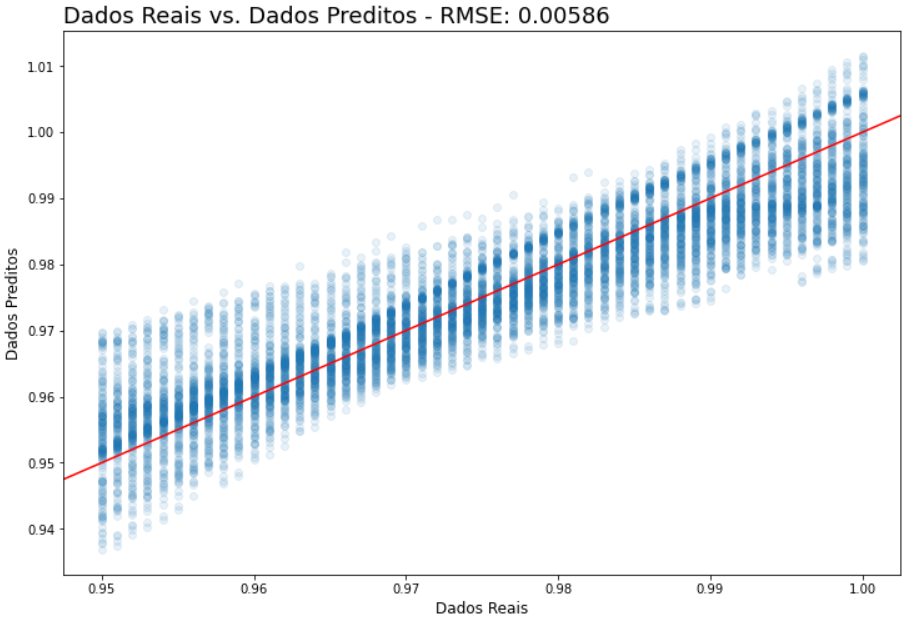
\includegraphics[width=9.7cm]{treinoGT}
  \caption{Resultado da predição de treino para a variável dependente $GTC$.}
  \label{fig:treinoGT}
\end{figure}

\begin{figure}[h]
  \centering
  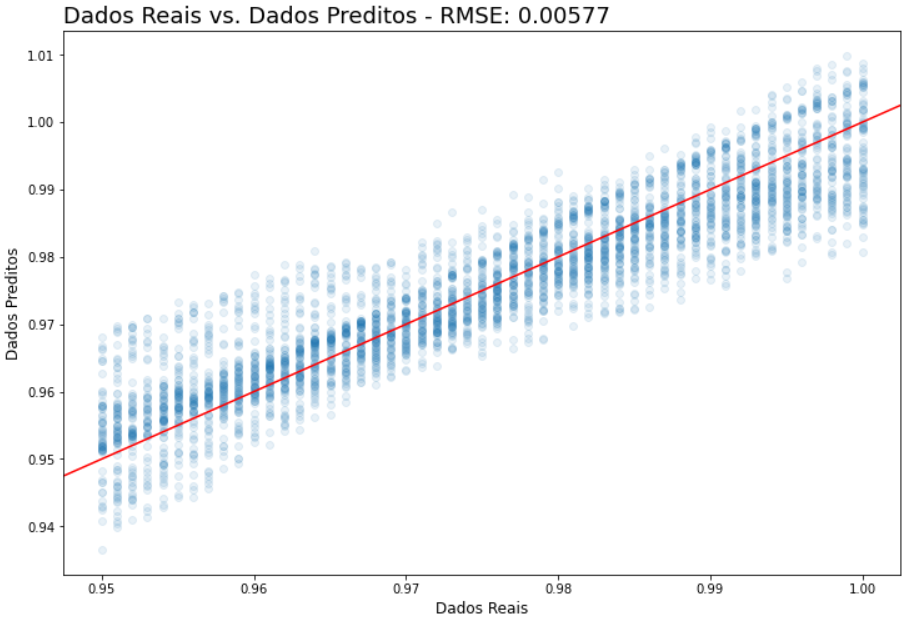
\includegraphics[width=9.7cm]{testeGT}
  \caption{Resultado da predição de teste para a variável dependente $GTC$.}
  \label{fig:testeGT}
\end{figure}

Para a segunda variável dependente $GTT$:

\begin{figure}
  \centering
  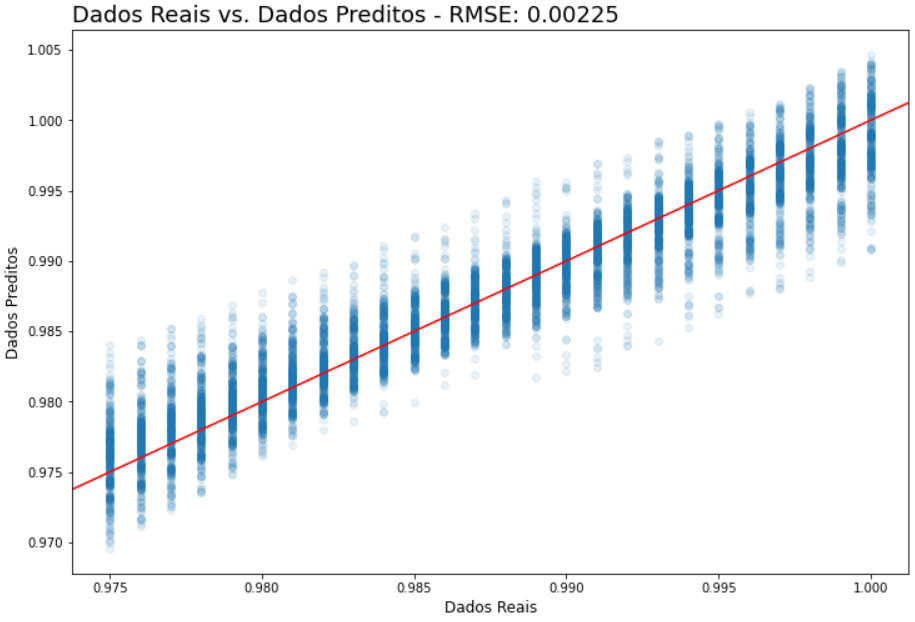
\includegraphics[width=9.7cm]{treinoGT1}
  \caption{Resultado da predição de treino para a variável dependente $GTT$.}
  \label{fig:treinoGT1}
\end{figure}

\begin{figure}
  \centering
  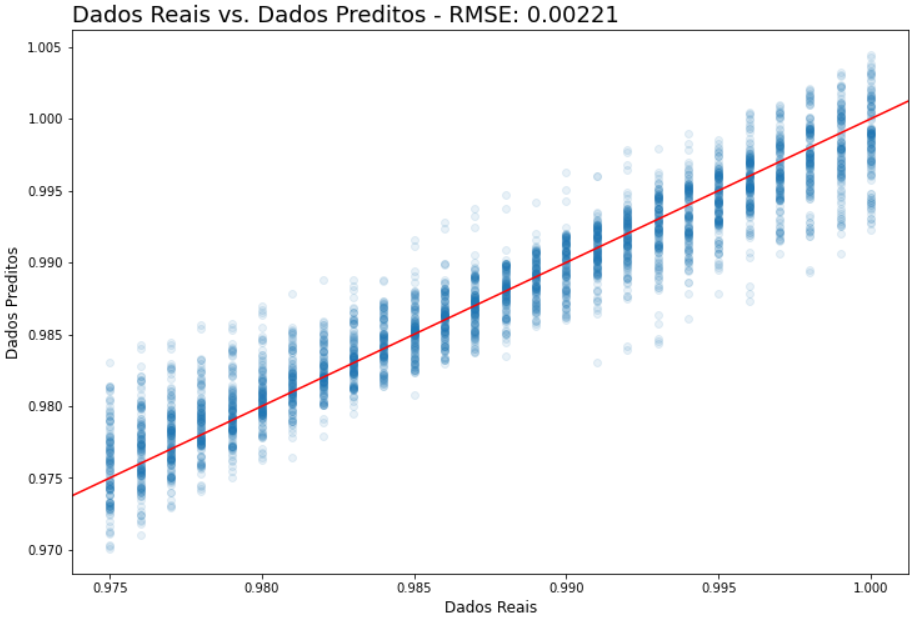
\includegraphics[width=9.7cm]{testeGT1}
  \caption{Resultado da predição de teste para a variável dependente $GTT$.}
  \label{fig:testeGT1}
\end{figure}


\newpage
\section{Conclusão}

A solução de uma regressão linear com o método dos mínimos quadrados é uma tarefa utilizada em diversas aplicações, com importância para os mais variados nichos do conhecimento, aliando simplicidade e robustez em sua solução.

Já para os experimentos realizados para o conjunto de dados sobre a indústria naval, concluímos que a regressão linear com o método dos mínimos quadrados resolvido com a decomposição QR nos dá uma estimativa e previsão relativamente boas o suficiente das duas variáveis dependentes utilizadas.

\newpage
\section{Trabalhos Futuros}

Futuros trabalhos podem se aprofundar ainda mais no método de regressão linear para o problema em questão da indústria naval, buscando qual combinação de variáveis diminui a métrica RMSE em teste. Por exemplo, se usarmos apenas 5 das 16 variáveis, o erro irá diminuir ou aumentar? Quais variáveis mais influenciam e se correlacionam com o valor final de $GTC$ e $GTT$?

\newpage
\section{Referências Bibliográficas}

\nocite{reamat}
\nocite{Coraddu2013Machine}
\nocite{gram-notes}

\printbibliography[heading=none]




\end{document}